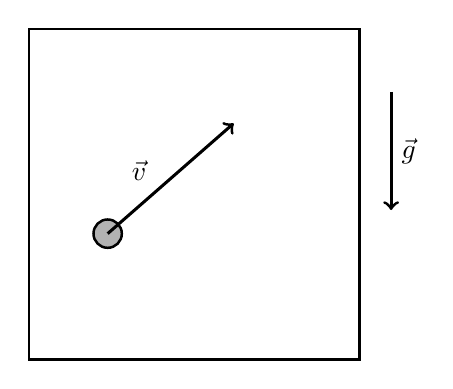
\begin{tikzpicture}[line width=0.9pt]
  % bounding box
  \draw (0,0) rectangle (4.2,4.2);
  % ball
  \filldraw[fill=gray!60] (1.0,1.6) circle (0.18);
  % velocity vector v
  \draw[->, line width=1.1pt] (1.0,1.6) -- (2.6,3.0);
  \node at (1.4,2.4) {$\vec{v}$};
  % gravity vector g outside the box, on the right
  \draw[->, line width=1.1pt] (4.6,3.4) -- (4.6,1.9);
  \node[right] at (4.6,2.65) {$\vec{g}$};
\end{tikzpicture}
